\title{Bugs in winter}

\author{by John Hudson and Bob Armstrong}

\maketitle

\begin{figure}[H]
\begin{center}
%\vspace{2mm}
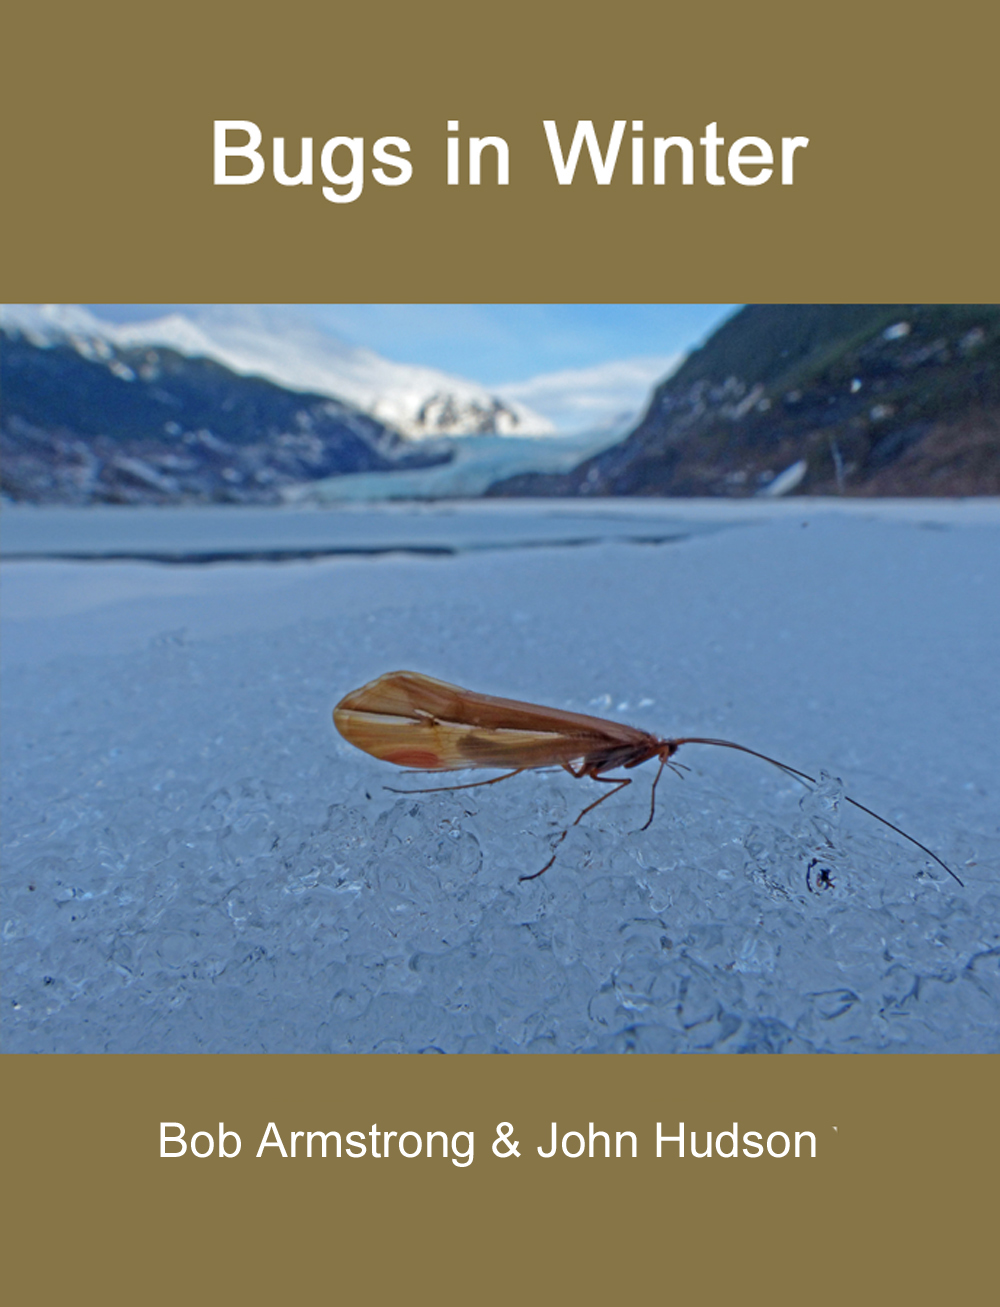
\includegraphics[width=\textwidth]{img/bugs_in_winter.jpg}
\caption{Cover of the \textit{Bugs in Winter} guide.}
\label{bugs_in_winter}
\end{center}
\end{figure}

We got started on ``\textit{Bugs in Winter}'' (Figure \ref{bugs_in_winter}), a small guide to some of the invertebrates seen around Juneau in winter, when we noticed tiny springtails moving about on the surface of the snow (Figure \ref{Ptenothrix}). And then we saw and photographed a beetle larva (Figure \ref{Cantharidae}) and adult dance fly (Figure \ref{dance_fly}) eating a springtail on the snow in mid-winter. These events stimulated our interest and desire to learn and understand why some bugs are out and about in winter. For example, one study indicated that some springtails are able to move fairly long distances, about a mile, on the snow by orientating on the sun or the dark horizon (something they can't do living down in and on the ground in summer).

\begin{figure}[H]
\begin{center}
\vspace{2mm}
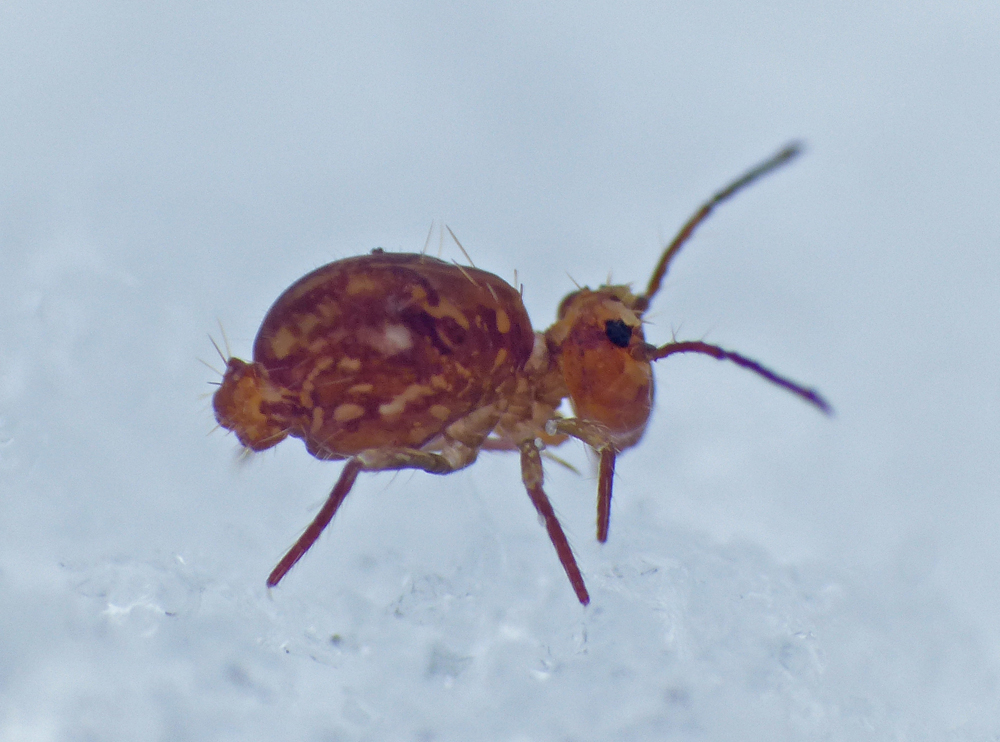
\includegraphics[width=\textwidth]{img/Ptenothrix.jpg}
\caption{A springtail in the Genus \textit{Ptenothrix} identified by Frans Janssens.}
\label{Ptenothrix}
\end{center}
\end{figure}

\end{multicols}
\begin{figure}[H]
\begin{center}
\vspace{2mm}
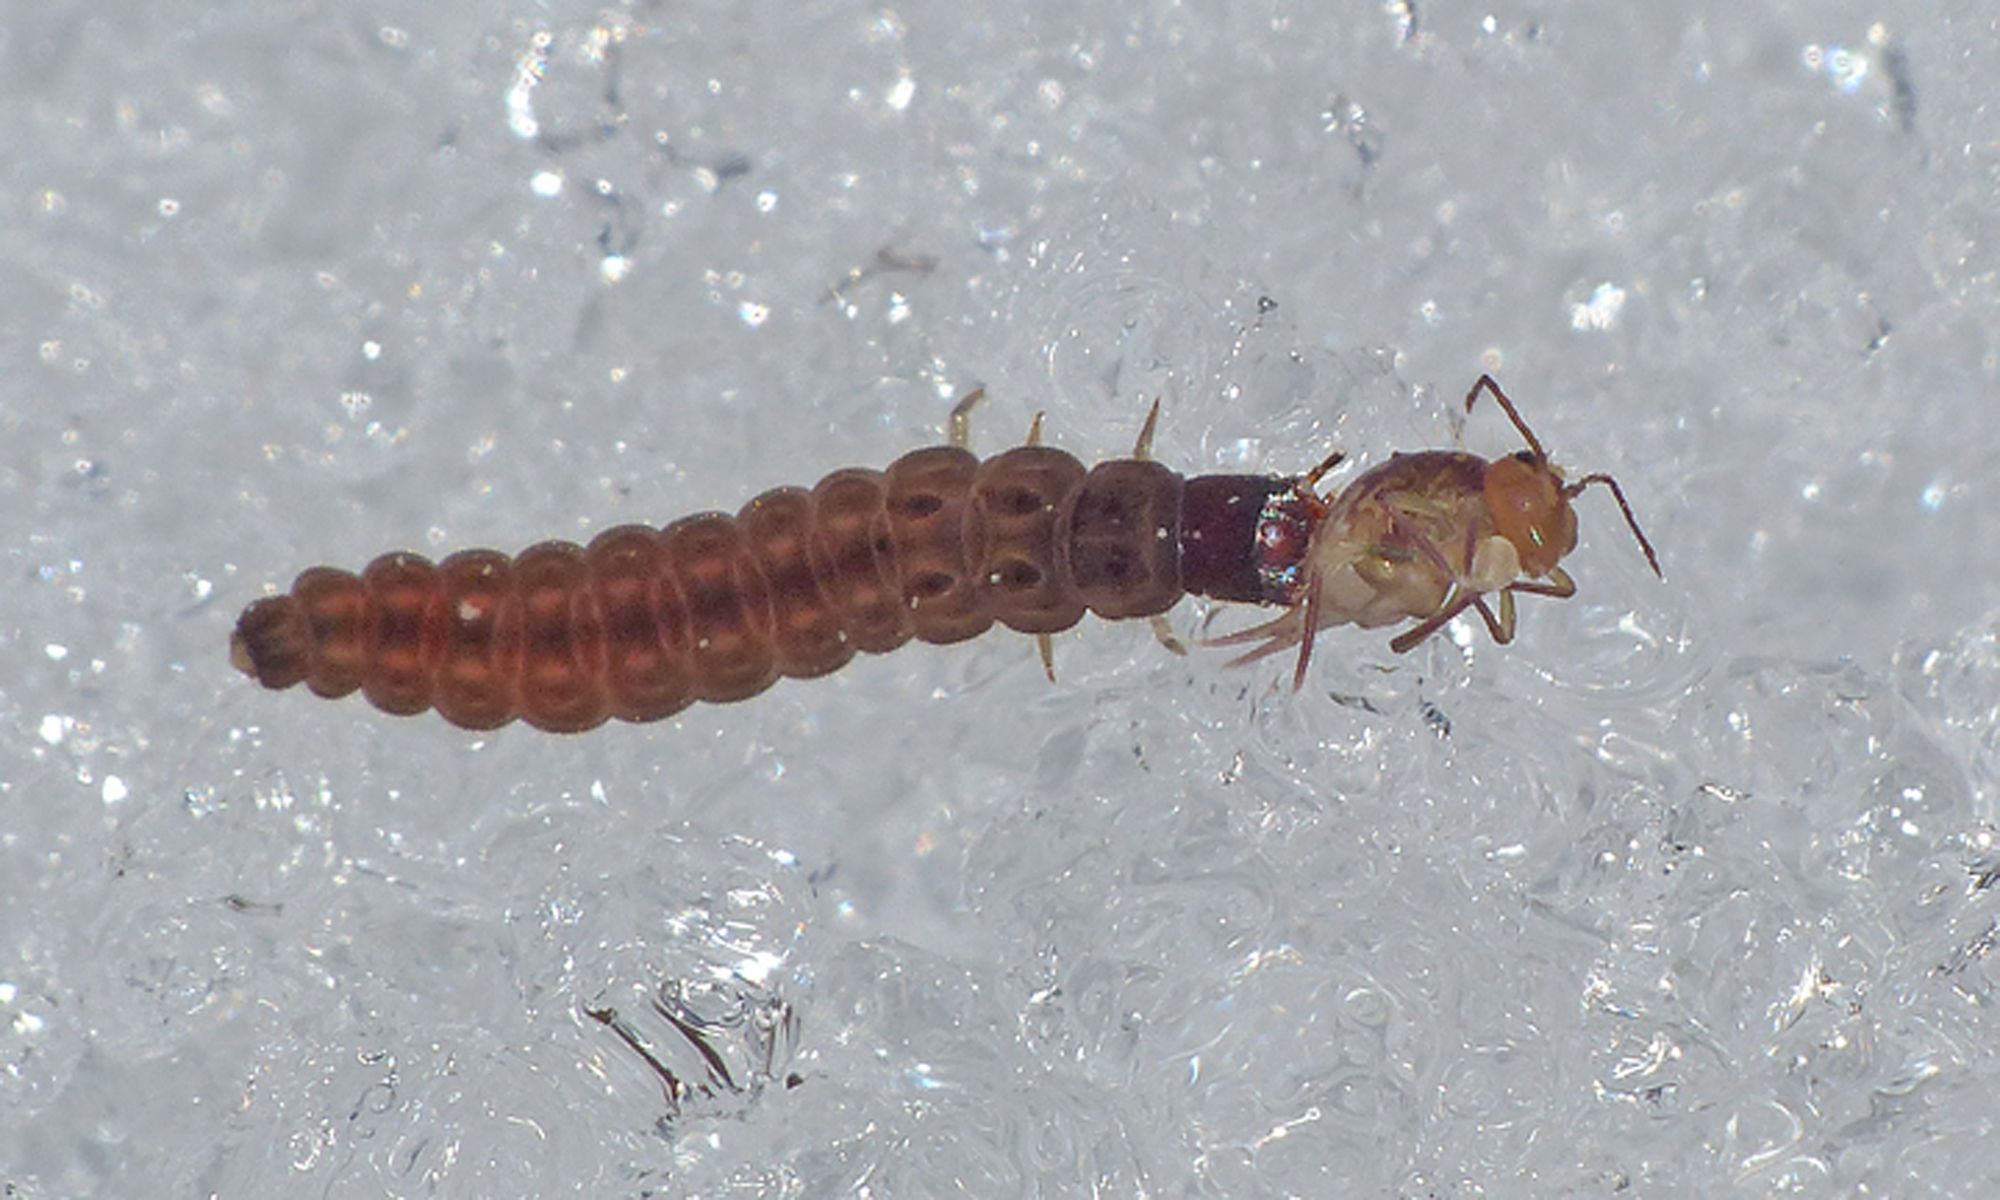
\includegraphics[width=\textwidth]{img/Cantharidae.jpg}
\caption{A soldier beetle larva (Family Cantharidae) feeds on a springtail.}
\label{Cantharidae}
\end{center}
\end{figure} 
\begin{multicols}{2}

\begin{figure}[H]
\begin{center}
\vspace{2mm}
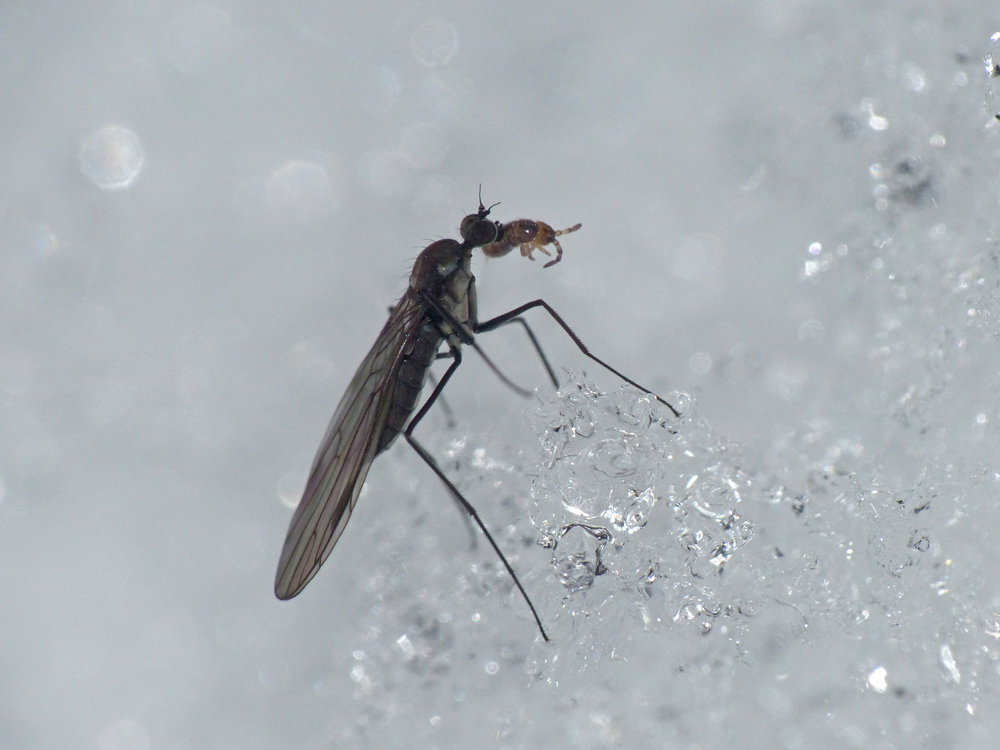
\includegraphics[width=\textwidth]{img/dance_fly.jpg}
\caption{An adult dance fly feeds on a springtail.}
\label{dance_fly}
\end{center}
\end{figure}

The good news is there are a broad range of invertebrates that are active in winter, but not too many. So, it was possible to put together photos and information that covers the ones you are most likely to see. Our little \textit{Bugs in Winter} guide contains interesting facts about the creatures and their behavior. You can see what we have learned so far in this evolving pdf: \url{https://www.naturebob.com/sites/default/files/Bugs%20in%20Winter%20optimized%20March%201%2C%202021.pdf}. Our main reason for creating Bugs in Winter is to provide information to educators to inform and stimulate their students about the variety of invertebrates that can be easily seen on snow in winter. 

In winter we often see spiders crawling about on the snow (Figure \ref{Pityohyphantes}). Some of the spiders appeared to be frozen. Spiders are freeze resistant but not freeze tolerant. Several spiders that appeared to be frozen were warmed gradually but did not ``come back to life.'' According to Joey Slowik, spiders that are on the snow during a warm period may be prevented from accessing refuges in leaf litter when the temperature suddenly falls below freezing. This may be the main reason that some become frozen on the snow surface.

\begin{figure}[H]
\begin{center}
\vspace{2mm}
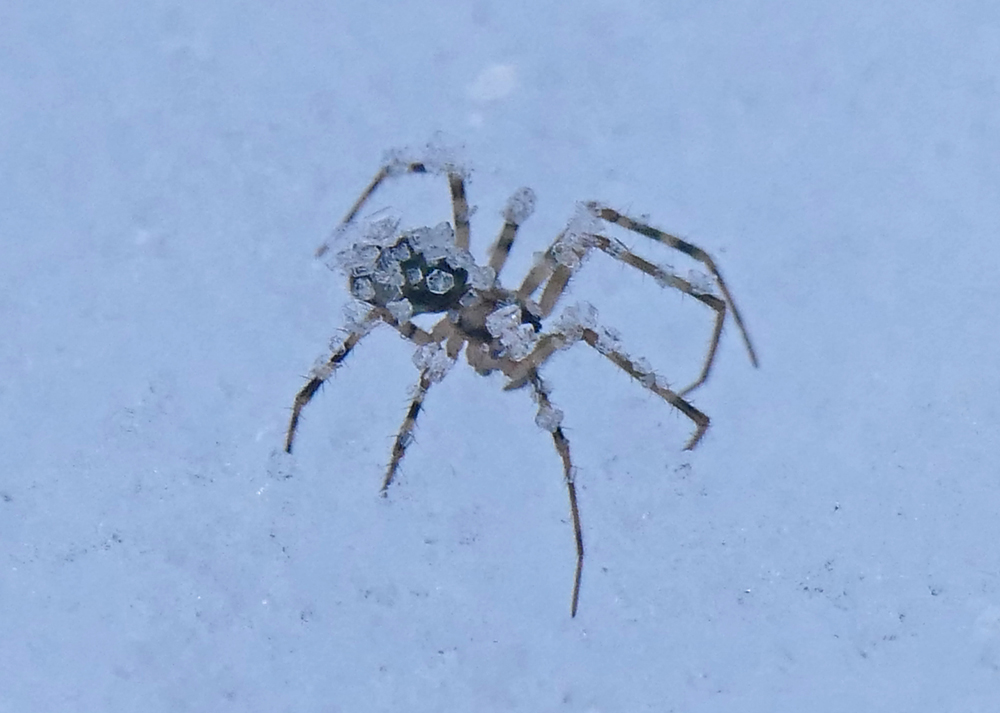
\includegraphics[width=\textwidth]{img/Pityohyphantes.jpg}
\caption{A frozen hammock spider (Genus \textit{Pityohyphantes}, identified by Joey Slowik).}
\label{Pityohyphantes}
\end{center}
\end{figure}

The Bruce spanworm moth is well known for outbreaks that can defoliate leaves of deciduous trees and shrubs throughout much of Alaska. In Juneau we see the males mating at night with the wingless females on blueberry plants in late fall and early winter (Figure \ref{bruce_spanworm}). Eggs are laid near the plants and the caterpillars emerge in spring and feed on the blueberry leaves. One study indicated that the defoliation by Bruce spanworms on blueberries may, over the long run, actually benefit the plants. It appears that the caterpillars’ frass provides more nutrients than the autumn-shed leaves.

At Nugget Falls near the Mendenhall Glacier we often see adult midges (Family Chironomidae) mating on snow and ice in mid-winter. Some of these midges are commonly called snow midges (genus \textit{Diamesa}, Figure \ref{Chironomidae}). Snow midges are one of the first insects to colonize streams exposed by retreating glaciers. Some adults can survive temperatures down to 3~\textdegree{}F, but quickly die if held in a warm hand.

The vast majority of caddisflies (order Trichoptera) overwinter in the egg or larval stage. A few caddisflies overwinter as adults and are referred to as snow sedges. The snow sedge \textit{Psychoglypha subborealis} is often seen flying on pleasant days in late fall and early spring, even when there is snow on the ground in Juneau (Figure \ref{snow_sedge}). The larvae of this caddisfly are often found in water bodies that shrink in size or dry up in winter. Safe inside the overwintering adult, the eggs avoid exposure to harsh winter conditions. 

\begin{figure}[H]
\begin{center}
\vspace{2mm}
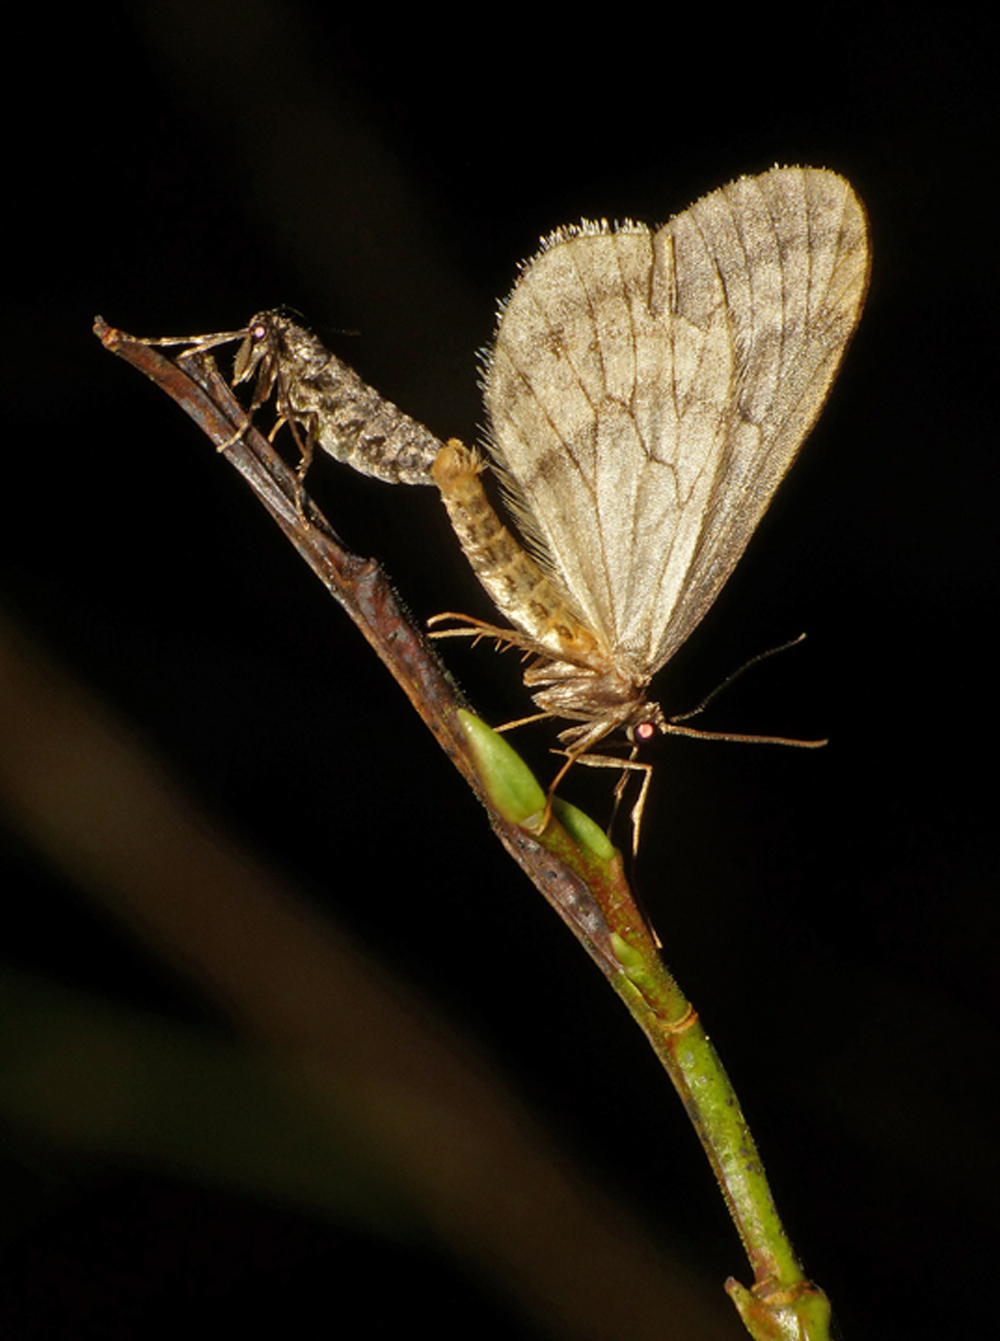
\includegraphics[width=\textwidth]{img/bruce_spanworm.jpg}
\caption{A male Bruce spanworm mates with the wingless female.}
\label{bruce_spanworm}
\end{center}
\end{figure}


\end{multicols}
\begin{figure}[H]
\begin{center}
\vspace{2mm}
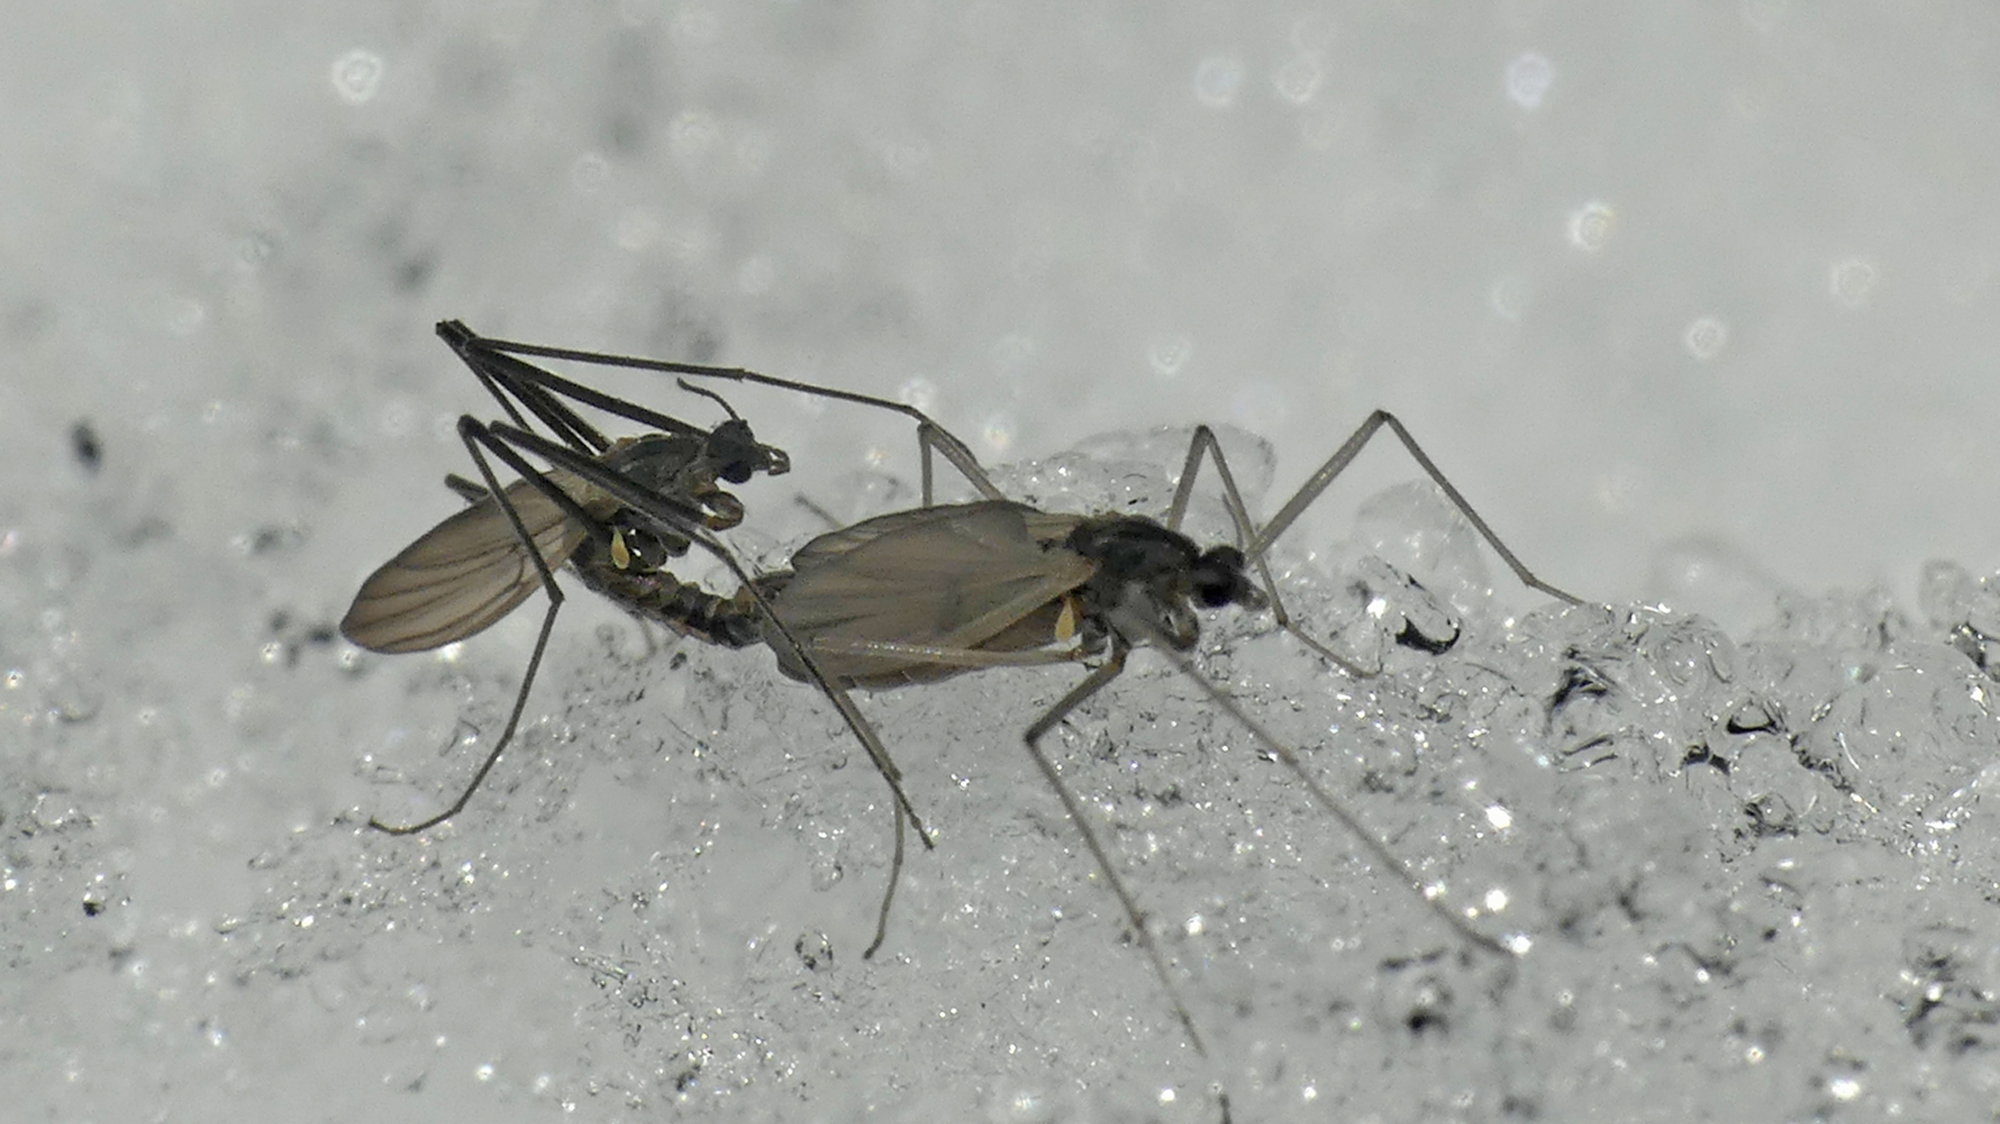
\includegraphics[width=\textwidth]{img/Chironomidae.jpg}
\caption{A mating pair of non-biting midges in the Genus \textit{Diamesa}.}
\label{Chironomidae}
\end{center}
\end{figure} 
\begin{multicols}{2}



\begin{figure}[H]
\begin{center}
\vspace{2mm}
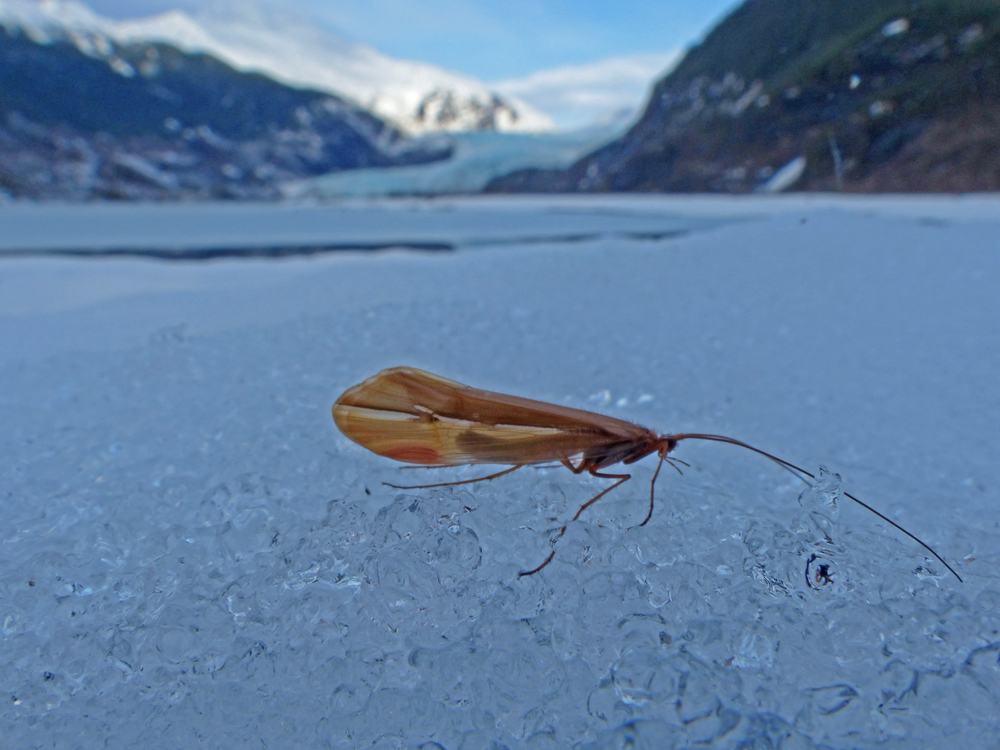
\includegraphics[width=\textwidth]{img/snow_sedge.jpg}
\caption{The snow sedge \textit{Psychoglypha subborealis} near the Mendenhall Glacier in Juneau.}
\label{snow_sedge}
\end{center}
\end{figure}

One of the most common and easily observed winter-active insects are the snowflies. Snowflies belong to a few families in the order Plecoptera (stoneflies). Adults emerge in late winter and crawl about on the snow in search of mates (Figure \ref{Capniidae}). Unlike other stoneflies, snowflies do not fly despite having wings. In some the wings are reduced or absent. Bridges, poles, and fences near streams are great places to find adult snowflies.

Acknowledgement: We would like to thank Derek Sikes for identifying the soldier beetle, Joey Slowik for identifying the hammock spider and Frans Janssens for identifying the springtail.

\end{multicols}
\begin{figure}[H]
\begin{center}
\vspace{2mm}
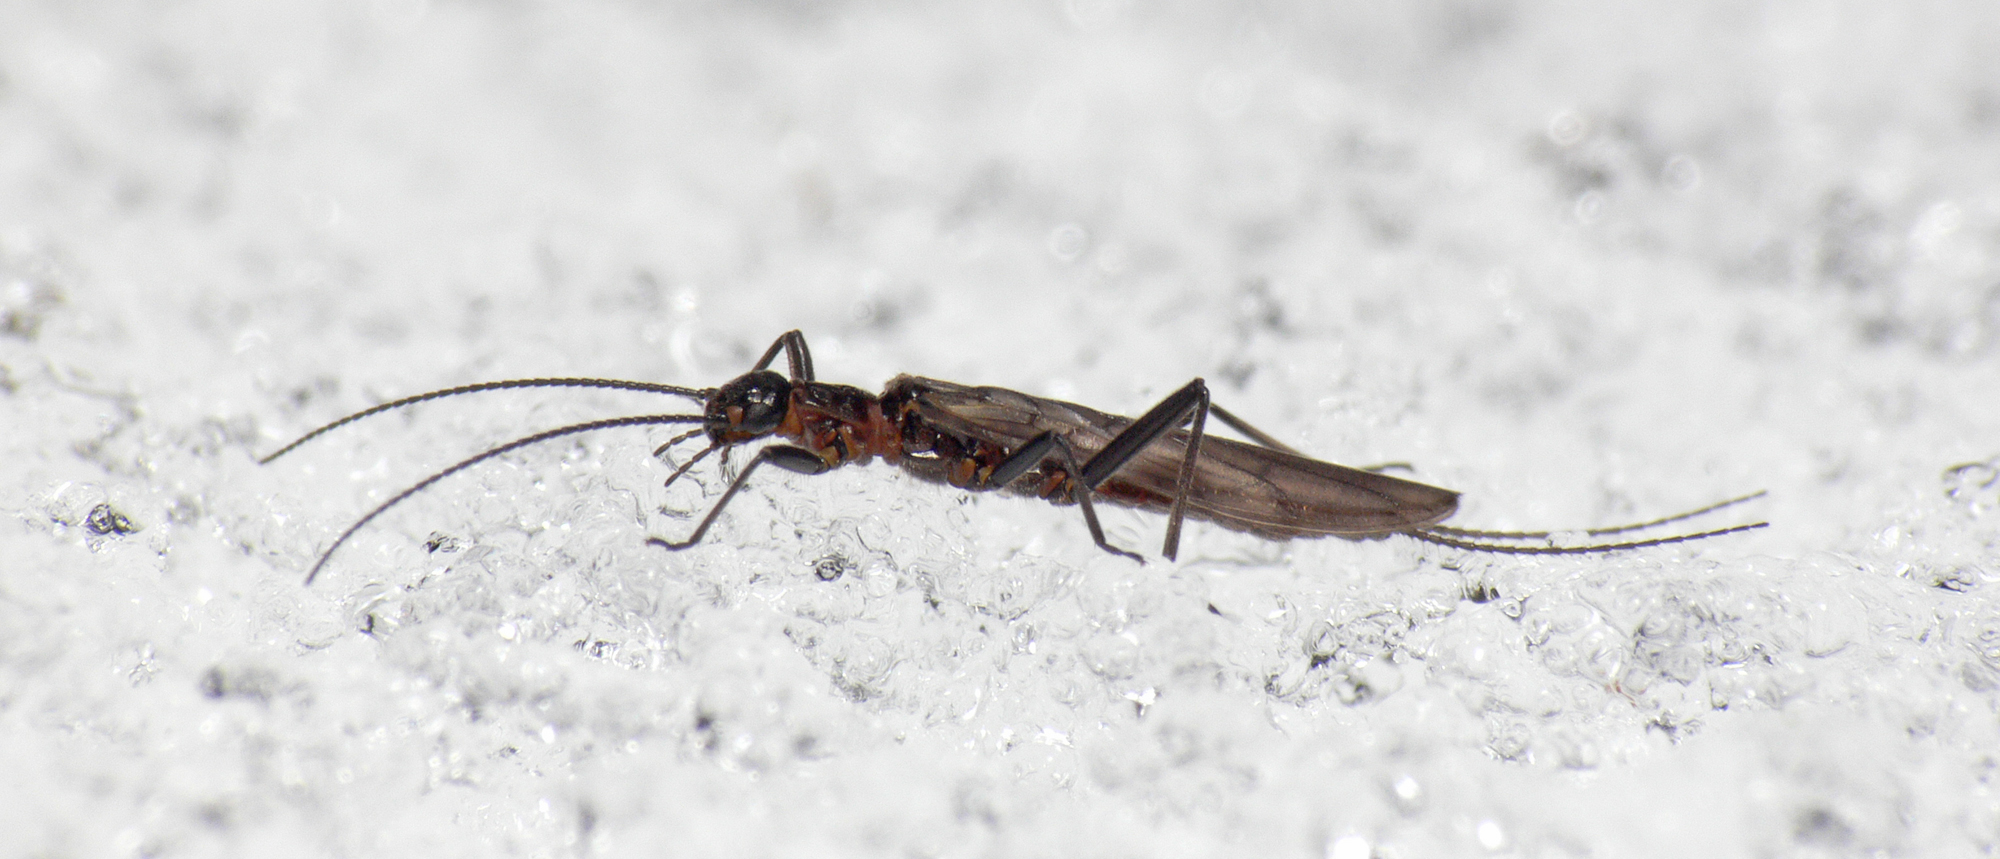
\includegraphics[width=\textwidth]{img/Capniidae.jpg}
\caption{An adult snowfly (Family Capniidae).}
\label{Capniidae}
\end{center}
\end{figure} 
\begin{multicols}{2}

